% Clocks that run fastest in the middle: alpha = 1 + (1/2) exp(-x^2) (top),
% and the transverse stress demanded, p_y = alpha''/(8 pi alpha), shown as
% alpha''/alpha (bottom): tension (red) where alpha'' < 0, pressure (blue)
% where alpha'' > 0. Here alpha'' = (1/2) exp(-x^2) (4x^2 - 2).
\documentclass[tikz,border=1pt]{standalone}
% Shared preamble for the standalone figures: the book's fonts, palette and
% drawing styles. Figures are drawn at their final printed size. A column is
% 3.35in (241pt) wide; a figure across both columns is 7in (505pt) wide.

\usepackage[T1]{fontenc}
\usepackage{newpxtext}
\usepackage[varbb]{newpxmath}
\usepackage[semibold,scale=0.95,lining]{sourcesanspro}
\usepackage{xcolor}
% Palette shared by the book and by the standalone figures in figures/src.
% One main hue (blue), one accent (orange), and a few roles used sparingly.

\definecolor{seblue}{HTML}{1D5B8F}    % headings, worked examples, main curves
\definecolor{seblueDark}{HTML}{123E63}
\definecolor{seorange}{HTML}{DC7A26}  % thought experiments, light and light cones
\definecolor{seteal}{HTML}{1F8577}    % checks, travellers and ships
\definecolor{sered}{HTML}{C0392B}     % negative energy, tension, violations
\definecolor{seviolet}{HTML}{5E548E}  % going deeper
\definecolor{sesand}{HTML}{8C6A3F}    % history
\definecolor{segray}{HTML}{6B7480}    % axes, guides, secondary labels
\definecolor{selight}{HTML}{D5DAE1}   % grids and faint rules

\usepackage{siunitx}
\usepackage{fontawesome5}
\usepackage{tikz}
\usetikzlibrary{arrows.meta,calc,positioning,decorations.pathreplacing,
  decorations.markings,shapes.geometric,fadings,shadings,patterns,3d,
  intersections,backgrounds}
\usepackage{pgfplots}
\pgfplotsset{compat=1.18}
\usepgfplotslibrary{fillbetween,groupplots,colormaps}

\tikzset{
  >={Latex[length=2.1mm,width=1.4mm]},
  every picture/.style={line cap=round, line join=round},
  lbl/.style={font=\sffamily\footnotesize, text=black!85},
  smalllbl/.style={font=\sffamily\scriptsize, text=black!75},
  guide/.style={segray, line width=0.4pt},
  axisline/.style={segray, line width=0.5pt, -{Latex[length=1.7mm,width=1.1mm]}},
  light/.style={seorange, line width=0.9pt},
  lightdash/.style={seorange, line width=0.9pt, dash pattern=on 3pt off 2pt},
  ship/.style={seteal, line width=1.4pt},
  cone/.style={fill=seorange!22, draw=seorange!85!black, line width=0.35pt},
}

\pgfplotsset{
  se axis/.style={
    axis lines=left,
    axis line style={segray, line width=0.5pt, -{Latex[length=1.6mm,width=1.1mm]}},
    tick style={segray, line width=0.4pt},
    major tick length=2.5pt,
    tick label style={font=\sffamily\scriptsize, text=black!75},
    label style={font=\sffamily\footnotesize, text=black!85},
    every axis plot/.append style={line width=1.1pt},
    legend style={font=\sffamily\scriptsize, draw=none, fill=none},
    scaled ticks=false,
    xticklabel={\sansnum{\tick}}, yticklabel={\sansnum{\tick}},
  },
}

% Numbers in figures are set in the sans-serif text font, with a true minus.
\sisetup{mode=text, reset-text-family=false, reset-text-series=false,
  reset-text-shape=false, drop-zero-decimal, group-minimum-digits=5}
% Tick values arrive as long decimals (1.5000000000); parse them first.
\newcommand{\sansnum}[1]{\begingroup\pgfkeys{/pgf/fpu=false}%
  \pgfmathparse{1*(#1)}\num{\pgfmathresult}\endgroup}

\begin{document}
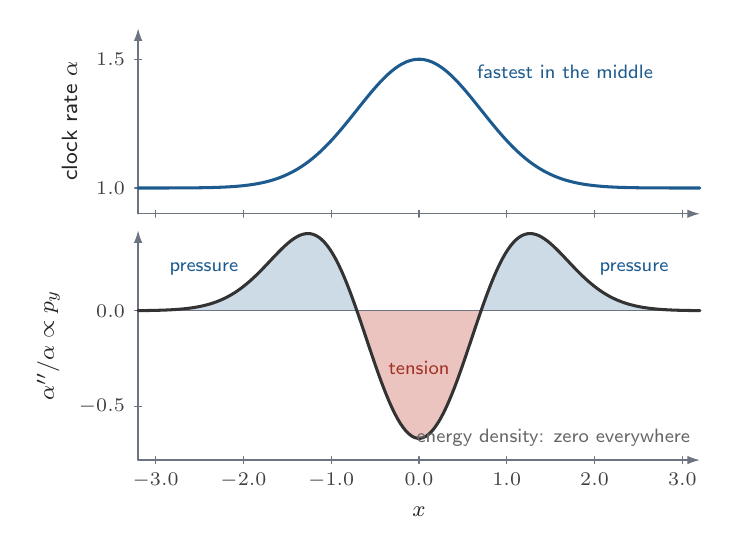
\begin{tikzpicture}
\begin{axis}[
  se axis, name=top, width=248pt, height=112pt,
  xmin=-3.2, xmax=3.2, ymin=0.9, ymax=1.62,
  xtick={-3,-2,-1,0,1,2,3}, xticklabels={}, ytick={1,1.5},
  ylabel={clock rate $\alpha$}, clip=false,
]
\addplot[seblue, domain=-3.2:3.2, samples=200] {1 + 0.5*exp(-x^2)};
\node[smalllbl, text=seblue, anchor=west] at (axis cs:0.55,1.45) {fastest in the middle};
\end{axis}
\begin{axis}[
  se axis, at={(top.south west)}, anchor=north west, yshift=-6pt,
  width=248pt, height=128pt,
  xmin=-3.2, xmax=3.2, ymin=-0.78, ymax=0.42,
  xtick={-3,-2,-1,0,1,2,3}, ytick={-0.5,0},
  xlabel={$x$}, ylabel={$\alpha''/\alpha \propto p_{y}$}, clip=false,
]
\addplot[draw=none, fill=sered!30, domain=-0.7071:0.7071, samples=80]
  {0.5*exp(-x^2)*(4*x^2 - 2)/(1 + 0.5*exp(-x^2))} \closedcycle;
\addplot[draw=none, fill=seblue!22, domain=0.7071:3.2, samples=80]
  {0.5*exp(-x^2)*(4*x^2 - 2)/(1 + 0.5*exp(-x^2))} \closedcycle;
\addplot[draw=none, fill=seblue!22, domain=-3.2:-0.7071, samples=80]
  {0.5*exp(-x^2)*(4*x^2 - 2)/(1 + 0.5*exp(-x^2))} \closedcycle;
\draw[segray, line width=0.4pt] (axis cs:-3.2,0) -- (axis cs:3.2,0);
\addplot[black!80, domain=-3.2:3.2, samples=200]
  {0.5*exp(-x^2)*(4*x^2 - 2)/(1 + 0.5*exp(-x^2))};
\node[smalllbl, text=sered!85!black] at (axis cs:0,-0.3) {tension};
\node[smalllbl, text=seblue] at (axis cs:2.45,0.22) {pressure};
\node[smalllbl, text=seblue] at (axis cs:-2.45,0.22) {pressure};
\node[smalllbl, text=black!60, anchor=south east] at (axis cs:3.2,-0.76) {energy density: zero everywhere};
\end{axis}
\end{tikzpicture}
\end{document}
